\chapter{Resultados} \label{cap6}
%\addcontentsline{toc}{chapter}{Resultados}

\begin{flushright}
\begin{minipage}{7.85cm}
    {\em Si buscas resultados distintos, no hagas siempre lo mismo.} \\ Albert
    Einstein
\end{minipage}
\end{flushright}

\vspace*{5mm}

\section{Preparación de la Simulación}

Para poder validar el trabajo realizado, hemos de simular lo ocurrido en el
caso guía y comparar los resultados con lo que realmente pasó. Para ello hemos
recopilado información de la inundación provocada por el paso del huracán
Katrina por Nueva Orleans en el año 2005.

Utilizando la información obtenida, creamos un escenario de simulación que
recrea la catástrofe que asoló la ciudad de Nueva Orleans. Como datos de
entrada utilizamos las roturas de los diques que contenían al río Mississippi
-nuestras Entradas de Agua-, la distribución de la población -los agentes
Peatón-, el terreno real y las calles reales de la ciudad.

\subsection{Áreas de Simulación}

El huracán Katrina afectó a una parte considerable del estado de Luisiana, pero
nosotros nos centraremos en la ciudad de Nueva Orleans. En concreto el área que
se inundó de la ciudad viene resaltada en la siguiente imagen.

\begin{figure}[H]
 \centering
 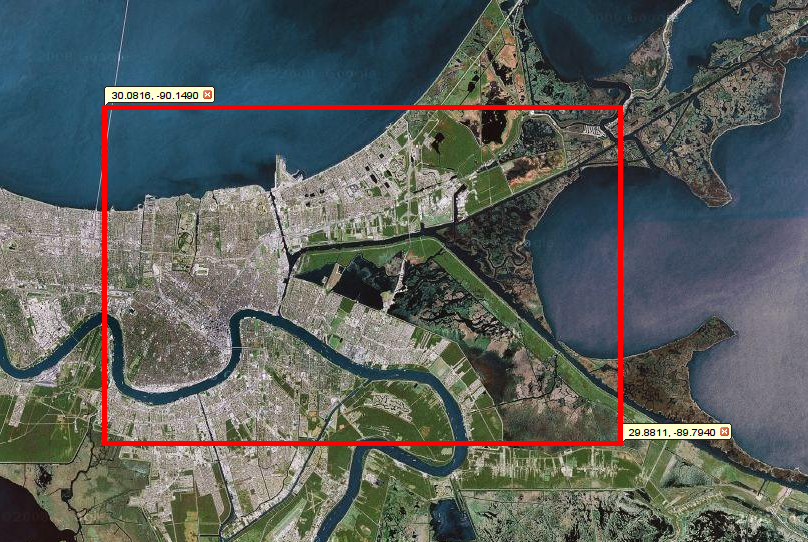
\includegraphics[height=120mm,angle=90]{figuras/cap6/NOarea1.png}
 \caption{Área de simulación}
\end{figure}

Al producirse la inundación por el desbordamiento del río, entre el mismo río y
los canales que atraviesan la ciudad dividieron la inundación en tres grandes
zonas casi independientes\cite{Pennington06}. En la siguiente imagen se puede
apreciar la división de la inundación en las tres zonas afectadas.

\begin{figure}[H]
 \centering
 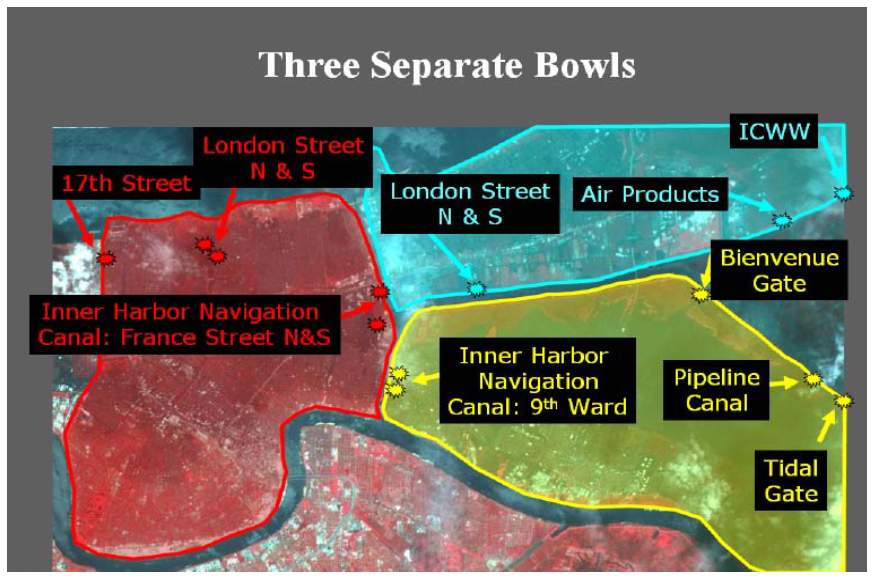
\includegraphics[width=100mm]{figuras/cap6/affected.png}
 \caption{División en 3 zonas del área afectada}
\end{figure}

Al ser el mismo río el que separa las diferentes zonas, éstas pueden simularse
por separado. Para ahorrar recursos y reducir la carga computacional nos
planteamos la creación de tres escenarios de simulación separados. Las
siguientes imágenes muestran las áreas de cada uno de dichos escenarios.

\begin{figure}[H]
 \centering
 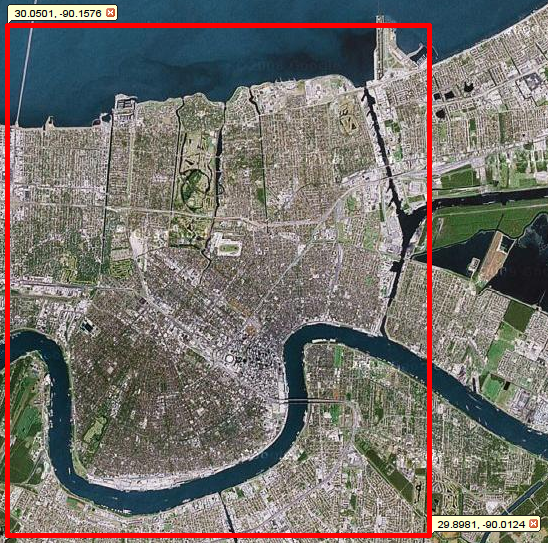
\includegraphics[width=120mm]{figuras/cap6/NOarea2.png}
 \caption{Zona 1 de simulación} \label{zona1}
\end{figure}

\begin{figure}[H]
 \centering
 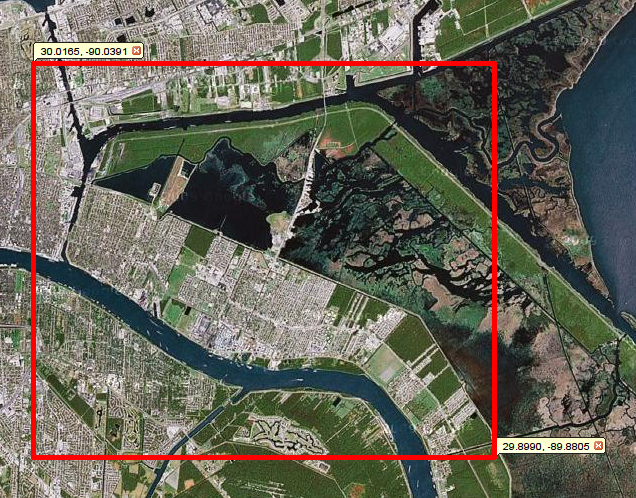
\includegraphics[width=135mm]{figuras/cap6/NOarea3.png}
 \caption{Zona 2 de simulación} \label{zona2}
\end{figure}

\begin{figure}[H]
 \centering
 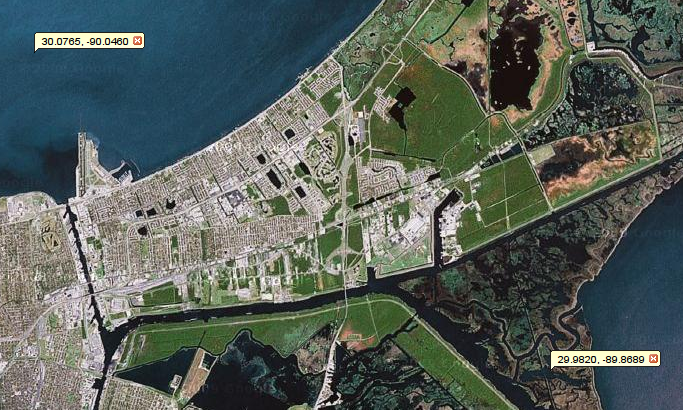
\includegraphics[width=135mm]{figuras/cap6/NOarea4.png}
 \caption{Zona 3 de simulación} \label{zona3}
\end{figure}

\subsection{Elevación del Terreno}

Para poder simular la inundación uno de los datos que tenemos que obtener es
la elevación del terreno. Para una zona tan grande como Nueva Orleans hacen
falta millones de datos de altura, sin embargo para nuestra simulación nos hemos
limitado a la parte de Nueva Orleans que resultó mas afectada, y hemos utilizado
hexágonos de 50 metros de tamaño.

Dado que el servicio web del que obtenemos la información nos obliga a
solicitar las alturas de las casillas una a una, y a que son muchísimas
casillas, la obtención de estos datos ha sido muy lenta. Es en estos casos
cuando la \hyperref[cache]{caché de alturas} demuestra su utilidad, dado que
nos permite ejecutar varias simulaciones sin tener que volver a descargar las
alturas.

\subsection{Roturas de los Diques}

La causa de que la ciudad se inundase fue que los diques no resistieron el paso
del huracán, se rompieron en múltiples localizaciones y el crecido Mississippi
anegó los barrios de la ciudad. Las posiciones\cite{Pennington06} de estas
roturas son las entradas de agua a la simulación.

\begin{figure}[H]
 \centering
 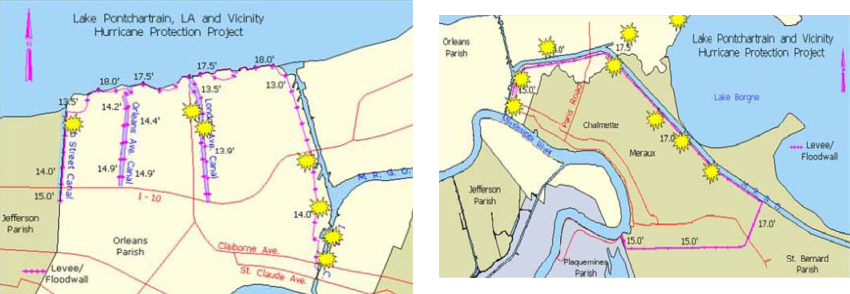
\includegraphics[width=135mm]{figuras/cap6/dikes.png}
 \caption{Localización de las roturas de los diques}
\end{figure}

En las siguientes imágenes se muestran geolocalizadas las posiciones de las
diferentes roturas que sufrieron los diques. En cada una de estas coordenadas
estará posicionado en la simulación un agente {\bf Entrada de Agua}.

\begin{figure}[H]
 \centering
 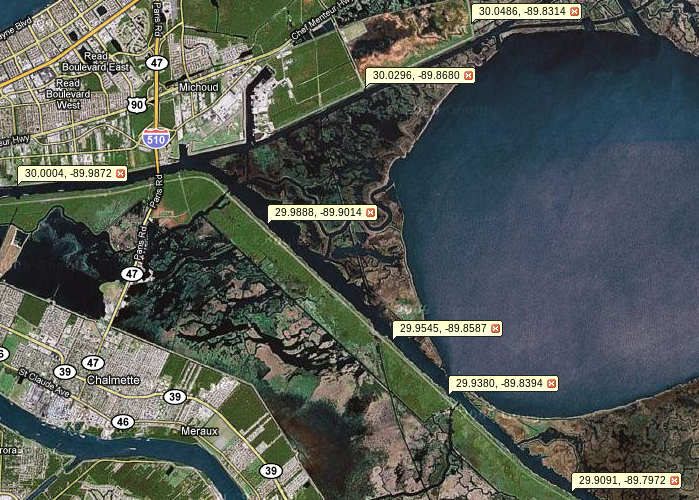
\includegraphics[width=135mm]{figuras/cap6/dikes1.png}
 \caption{Detalle de las roturas de los diques 1}
\end{figure}

\begin{figure}[H]
 \centering
 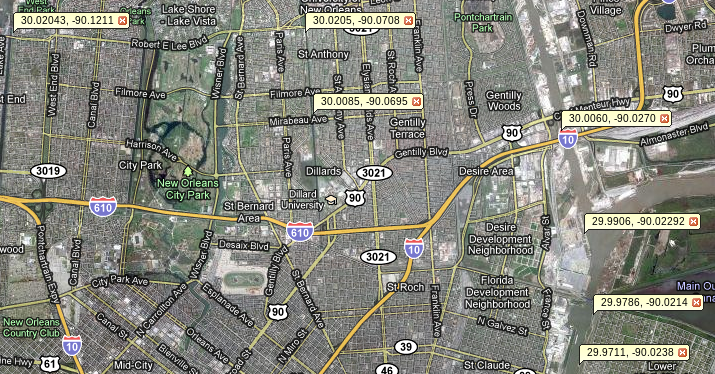
\includegraphics[width=135mm]{figuras/cap6/dikes2.png}
 \caption{Detalle de las roturas de los diques 2}
\end{figure}

\subsection{Distribución de la Población}

En las siguientes imágenes aparecen marcadas las posiciones sobre el mapa de
Nueva Orleans, de los agentes {\bf Peatón} que participan en la simulación.
Como se puede ver en los escenarios de simulación, en cada punto de inicio no
tiene por qué haber un único agente; de hecho, el número de clones del agente
que aparezca en uno de estos punto oscila entre 1 y 7.

\begin{figure}[H]
 \centering
 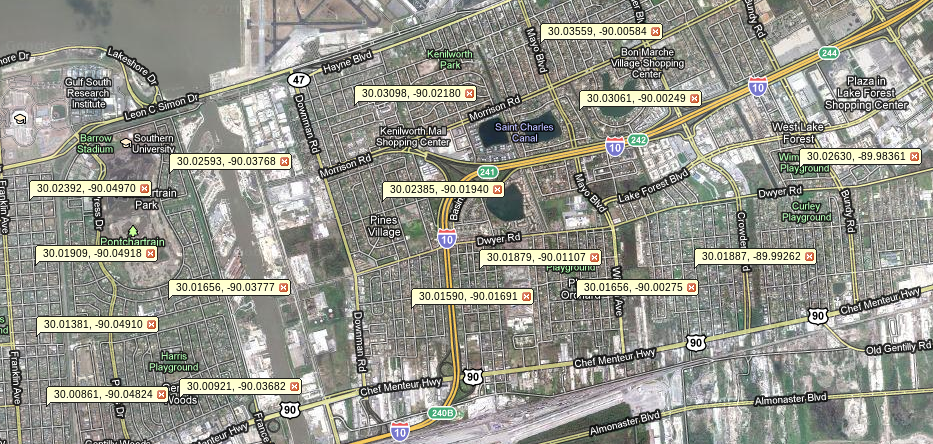
\includegraphics[height=90mm,angle=90]{figuras/cap6/population.png}
 \caption{Distribución de la población 1}
\end{figure}

\begin{figure}[H]
 \centering
 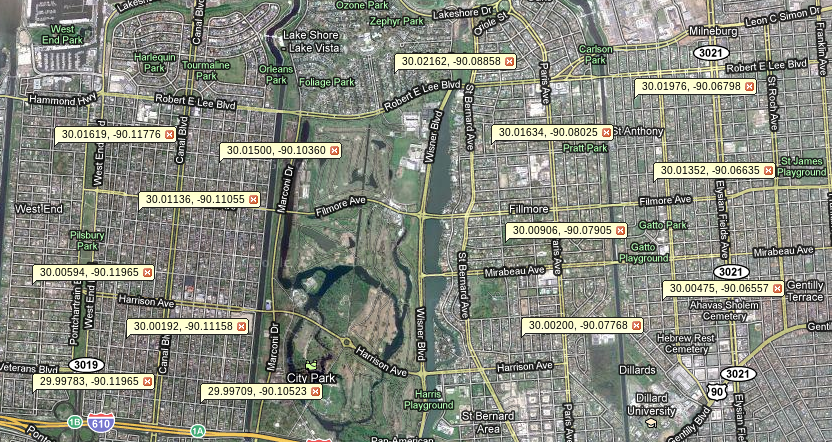
\includegraphics[height=90mm,angle=90]{figuras/cap6/population1.png}
 \caption{Distribución de la población 2}
\end{figure}

\begin{figure}[H]
 \centering
 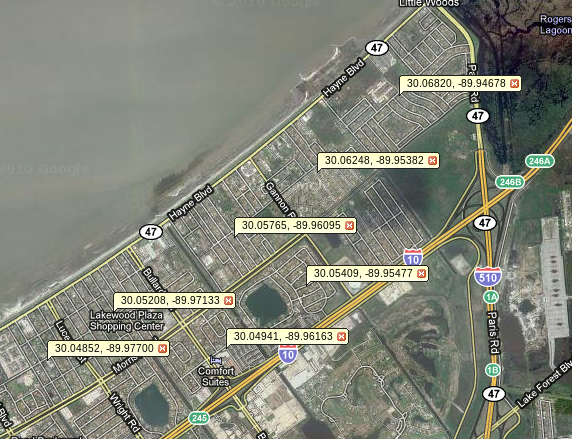
\includegraphics[width=120mm]{figuras/cap6/population2.png}
 \caption{Distribución de la población 3}
\end{figure}

\begin{figure}[H]
 \centering
 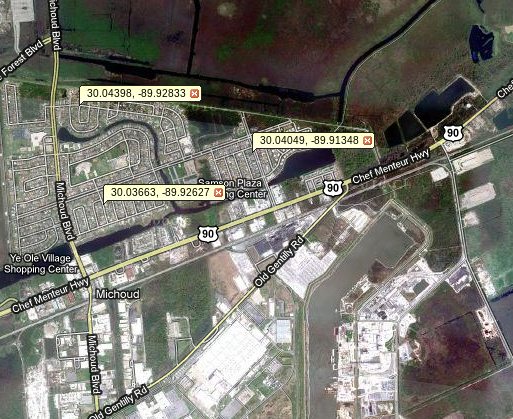
\includegraphics[width=105mm]{figuras/cap6/population3.png}
 \caption{Distribución de la población 4}
\end{figure}

\subsection{Refugios y Rutas de Evacuación}

En un principio se utilizó el {\em Louisiana Superdome} -una gran instalación
deportiva y de exhibición ubicada en el distrito central de negocios de Nueva
Orleans- como refugio, pero pasados unos días fue evacuado también. Dicha
instalación en encuentra en las coordenadas geográficas 29.950931°, -90.081364°.

Aparte del {\em Superdome}, no hubo otros refugios notables, si no que lo que se
hizo fue una evacuación completa de la ciudad. Por ello, hemos marcado como
objetivos tres posibles rutas de escape para los ciudadanos.

También consideramos que los edificios de los cuales podemos obtener
información a través de OSM pudieron ser refugios de emergencia donde
temporalmente pudieron refugiarse algunos ciudadanos.

En la siguiente imagen vienen marcados los objetivos de los agentes, son
refugios de los que conocen su posición desde un principio. Aunque si un agente
se encuentra con un refugio temporal de camino a un objetivo, correrá a
refugiarse y abandonará la búsqueda del objetivo.

\begin{figure}[H]
 \centering
 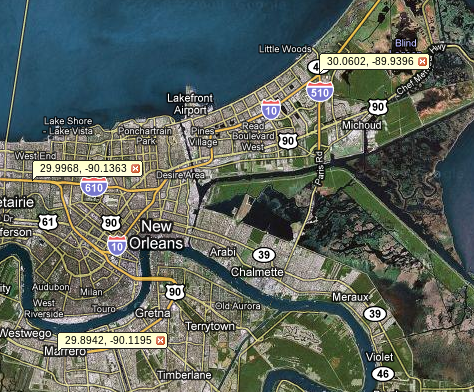
\includegraphics[width=105mm]{figuras/cap6/evacuation.png}
 \caption{Posibles rutas de evacuación y posición del Superdome}
 \label{objetivos}
\end{figure}

\subsection{Escenarios Simulados}

Con toda esta información recopilada hemos creado los escenarios para simular
la inundación posterior al huracán Katrina que asoló Nueva Orleans. A
continuación se lista el contenido de los ficheros de escenario para cada uno de
los tres barrios que hemos simulado.

Este primer escenario corresponde a \hyperref[zona1]{la zona 1} de simulación.
Se trata del {\em downtown} de Nueva Orleans, aunque también abarca zonas
residenciales. En el centro financiero hay edificios altos, incluso
rascacielos, lo que supone un contraste con el resto de la ciudad, más bien de
bajas alturas.

Aparte de las rutas de escape, en este barrio también se encuentra el {\em
Superdome} que consideramos un objetivo más. Contando con el {\em Superdome},
caen en este área de simulación dos \hyperref[objetivos]{objetivos}.

\lstinputlisting[caption=Escenario post Katrina simulado para la zona
1]{capitulo6/Katrina1.scen}

En este segundo barrio, bastante más pequeño, da la casualidad de que no
contiene ningún objetivo de los \hyperref[objetivos]{señalados anteriormente}.
Los agentes de este barrio tendrán, pues, que moverse por las calles de la
ciudad hasta dar con algún refugio donde resguardarse.

\lstinputlisting[caption=Escenario post Katrina simulado para la zona
2]{capitulo6/Katrina2.scen}

Los agentes del tercer y último barrio simulado conocen la posición de uno de
los \hyperref[objetivos]{objetivos}.

\lstinputlisting[caption=Escenario post Katrina simulado para la zona
3]{capitulo6/Katrina3.scen}

Como hora inicial hemos tomado las 9:00 AM del día 29 de Agosto de 2005, pues
fue cuando se produjo la primera rotura de uno de los diques de
contención\cite{DeLozier}.

\section{Resultados}

A la hora de simular un escenario tan inmenso nos hemos encontrado con
numerosos problemas, el enorme tamaño del área de simulación nos ha obligado a
buscar máquinas potentes con las que hacer la simulación.

Nuestros tutores nos brindaron la posibilidad de utilizar una máquina del
departamento, que cuenta con ocho núcleos de procesamiento. Por desgracia, no
tiene suficiente memoria como para manejar todos los datos, como descubrimos
amargamente al tratar de simular en dicha máquina.

Sacrificando la velocidad de procesado y en busca de mayor cantidad de memoria
migramos a otra máquina. La simulación se realizó en ordenador con las
siguientes características:

\begin{itemize}
 \item Dos núcleos de procesado a % TODO
 \item Cuatro gigas de memoria RAM
% TODO
\end{itemize}

\subsection{Visualización de Resultados}

Para la visualización de la inundación, como ya hemos comentado en varias
ocasiones, utilizamos un visor de ficheros KML. En concreto, utilizamos Google
Earth.

Gracias a la potencia de Google Earh podemos mostrar la inundación sobre
imágenes del terreno real y en 3 dimensiones.

\begin{figure}[H]
 \centering
 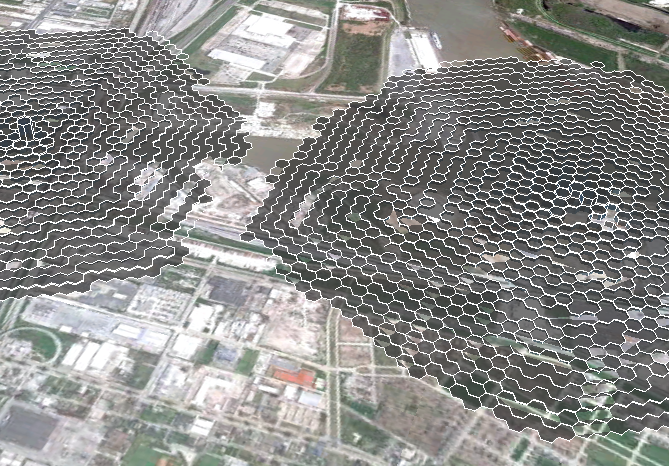
\includegraphics[width=110mm]{figuras/cap6/resultados/ejemplo.png}
 \caption{Dos fuentes de agua comienzan a inundar Nueva Orleans}
\end{figure}

\subsubsection{Interfaz de Google Earth}

A continuación vamos a explicar qué información podemos visualizar de los
ficheros KML a través de Google Earth. A la izquierda -marcada con un ``1'' en
la siguiente imagen- tenemos la barra lateral, en ella se despliega el
contenido del fichero KML que hemos abierto. Nos encontraremos con que en su
interior hay dos subcarpetas, {\em Flood} y {\em People}. En la primera se
almacenan los datos relativos al agua, mientras que en la segunda los relativos
a los peatones; todos ellos clasificados según entornos y con la hora
correspondiente.

Sobre el área principal -marcado con un ``2''- aparece el control de la
animación. Este control nos permite movernos a lo largo del tiempo visualizando
la inundación en todos sus estados, o bien podemos reproducirla y observar la
animación producida. También es posible modificar la velocidad a la que
muestra dicha animación.

El área principal -marcada con un ``3''- es donde Google Earth nos muestra el
mundo en 3D. Aquí es donde aparecerá dibujada la inundación. En la imagen
aparecen recuadradas las zonas que habían sido inundadas en el momento de tomar
la captura.

\begin{figure}[H]
 \centering
 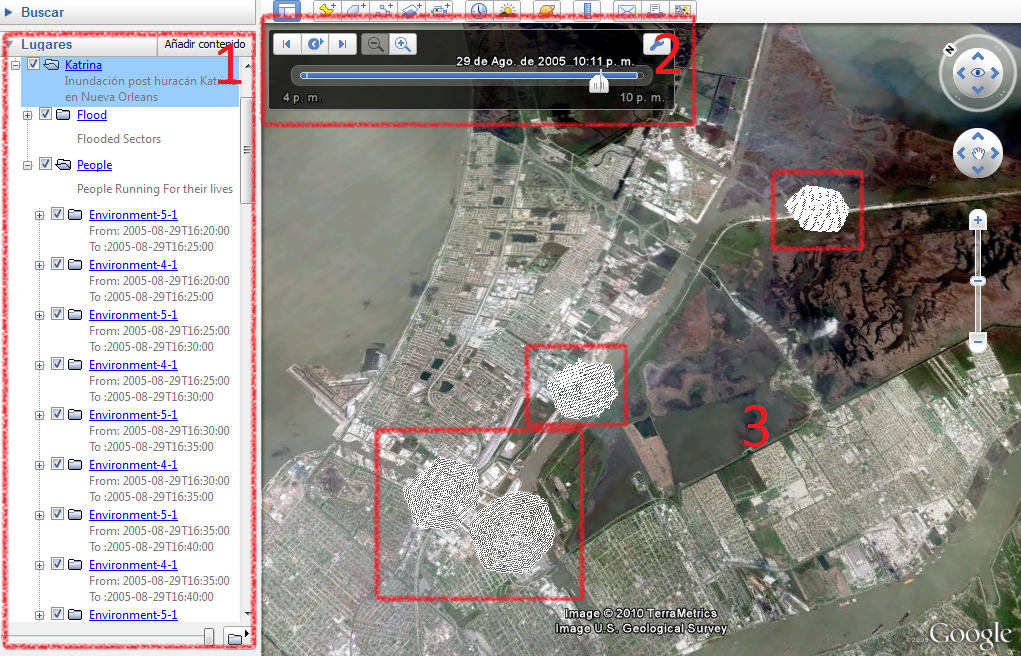
\includegraphics[height=130mm,angle=90]{figuras/cap6/resultados/interfaz.png}
 \caption{Interfaz de Google Earth}
\end{figure}

Entrando en detalle en la información almacenada en el KML, nos encontramos con
que respecto al agua -marcada con un ``1`` en la siguiente captura- se almacena
en cada instante de la simulación, y por cada entorno -marcado con un ''2''-, un
conjunto de polígonos -marcados con un ``3''- con un número asociado. Dicho
número es la altura del polígono en cuestión.

Podemos escoger en todo momento qué polígonos se muestran, y cuáles no. De esta
manera es muy intuitivo relacionar esta información con lo que está siendo
dibujado en la pantalla.

\begin{figure}[H]
 \centering
 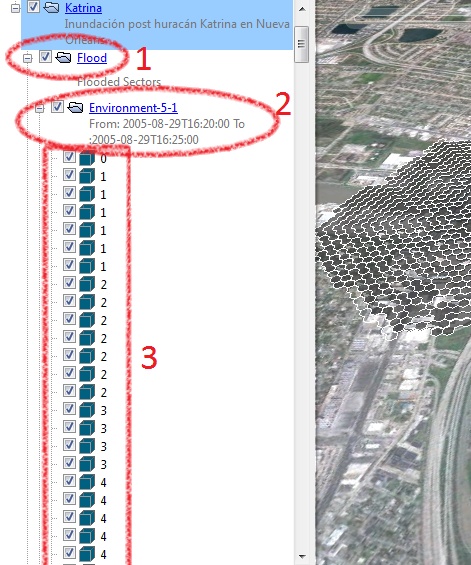
\includegraphics[width=95mm]{figuras/cap6/resultados/flood_data.png}
 \caption{Datos del agua en el KML}
\end{figure}

Al igual que ocurre con el agua, también podemos ver los detalles de la
información guardada sobre las personas -marcado con un ``1`` en la próxima
captura-. También aparecen clasificadas por entornos -marcados con un ''2``-, y
asociado a cada agente aparece un color y un número. El número es un cero, pues
siempre están caminando a ras de suelo. El color representa el estado del
agente:

\begin{description}
 \item[Amarillo] El agente está vivo, pero en peligro. Aún no ha encontrado
 ningún refugio.
 \item[Verde] El agente está a salvo en un refugio.
 \item[Gris] El agente ha muerto ahogado en la inundación.
\end{description}

Sobre el terreno se dibujan como un único hexágono -marcado con un ''3``-,
cuyas paredes son del color del estado del peatón.

\begin{figure}[H]
 \centering
 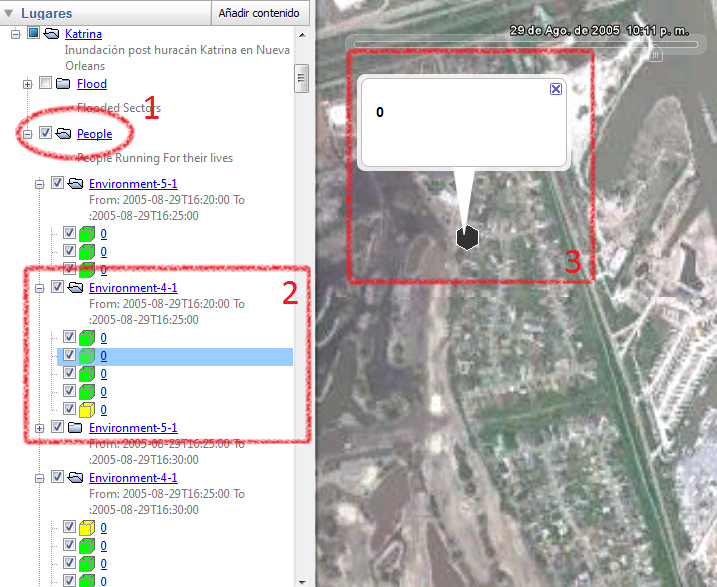
\includegraphics[width=130mm]{figuras/cap6/resultados/people_data.png}
 \caption{Datos de las personas en el KML}
\end{figure}

% TODO

\section{Simulación frente Realidad}
%Es cuestion de preparar un escenario de nueva orleans y comparar con la
%bibliografia

% TODO

En la siguiente imagen podemos observar qué zonas quedaron dañadas en Nueva
Orleans tras la inundación\cite{Gabe05}.

\begin{figure}[H]
 \centering
 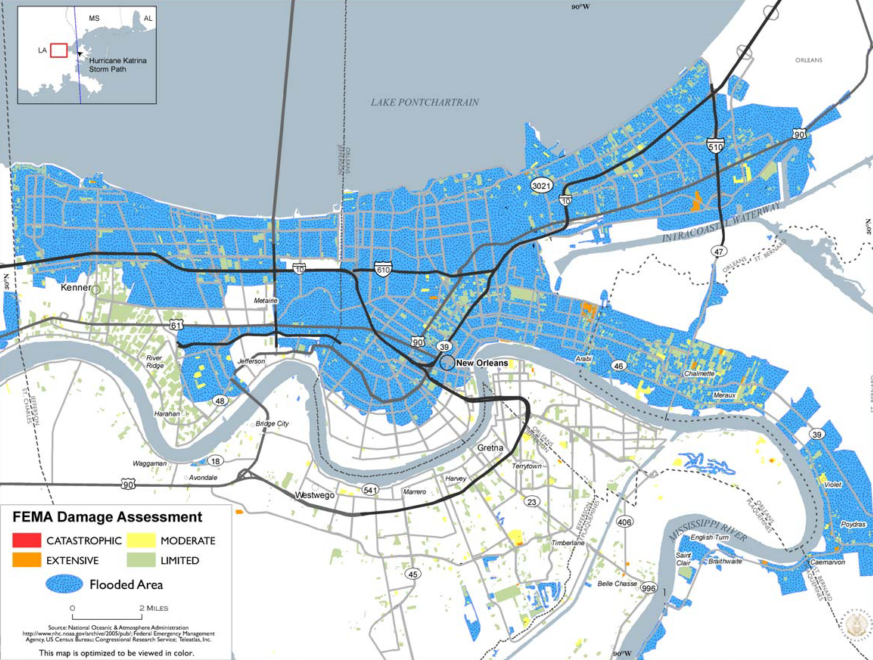
\includegraphics[width=135mm]{figuras/cap6/NOdamage.png}
 \caption{Daños reales en Nueva Orleans}
\end{figure}

%%% Local Variables:
%%% mode: latex
%%% TeX-master: "../dissim"
%%% End: